\subsection{Multijugador en \acf{UE4}}

Los juegos multijugador en \ac{UE4} son implementados bajo un enfoque basado en el modelo Cliente-Servidor. Esto significa que el servidor actúa como una \textbf{autoridad} y que todos los datos se deben enviar desde los distintos clientes, al servidor. El servidor valida los datos y reacciona a ellos. En \ac{UE4} se pueden distinguir dos tipos de servidores:

\begin{itemize}
\item \textbf{Servidor Dedicado}. Un servidor dedicado contiene una ventana de comandos en texto y no contiene los gráficos. Sin embargo carga el mundo, se ocupa de las físicas y fuerza que se cumplan las distintas reglas del juego. Además, un servidor dedicado no tiene jugadores locales, su función es conectar a distintos jugadores remotos en una misma partida, para que puedan jugar juntos. Los jugadores se conectan a un servidor dedicado a través de una dirección IP fija.

Para empaquetar y compilar el juego como un servidor dedicado, es necesario compilar el motor de \ac{UE4} desde los fuentes, que se pueden encontrar en \texttt{Github}\footnote{https://github.com/EpicGames/UnrealEngine}. Si el motor se ha instalado a través del instalador que proporciona Epic Games en su web\footnote{https://www.epicgames.com}, no será posible usar un servidor dedicado ya que Epic Games ha optado por no incluir algunos archivos en la versión que se descarga a través de su instalador debido al aumento de tamaño que producían. 

\item \textbf{\textit{Listen Server}}. Este tipo de servidor aloja un jugador local, pero permite también conexiones de jugadores remotos. Por tanto, en este modelo siempre habrá al menos un cliente conectado. Si este cliente se desconecta, el servidor se apaga. En este servidor se plantea el problema de que los jugadores que actúan como \textit{host} raramente tienen direcciones IP fijas a las que otros clientes puedan conectarse. Por este motivo, se desarrolló el \textbf{\textit{OnlineSubsystem}} (subsistema online), que se explicará más adelante. Este modelo elimina la latencia al jugador que actúa como \textit{host}.
\end{itemize}

En la Figura \ref{Objects}, se puede observar cómo es la distribución de los objetos en la arquitectura cliente-servidor implementada por \ac{UE4}. Ciertos objetos, como las interfaces gráficas, sólo existen en los clientes, mientras que otros como el \textit{GameMode} sólo existen en el servidor. Cabe destacar que en la intersección existente entre los dos clientes, no hay ningún objeto, ya que entre clientes no se comparte información que solo conozcan los clientes.

\begin{figure}[H]
  \centering
  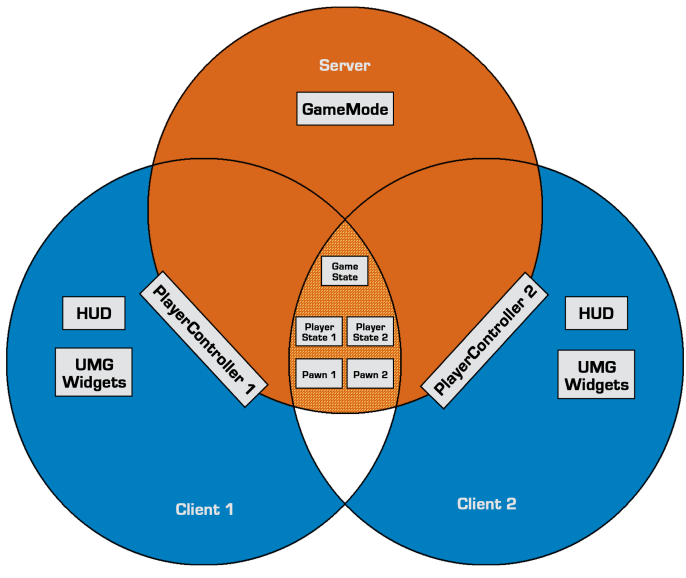
\includegraphics[width=10cm]{./images/ActorsInClientServer.png}
  \caption{Distribución de objetos en un enfoque Cliente-Servidor con \ac{UE4}}
  \label{Objects}
\end{figure}

Para que se pase información entre los clientes y el servidor, es necesaria la \textbf{replicación}. Replicar consiste en el envío de información y datos entre los clientes y el servidor. En \ac{UE4} se puede conseguir la replicación modificando características que afectan a los actores. Para que un actor se replique (aparezca en todos los clientes conectados al servidor) y su movimiento sea igualmente replicado, habrá que añadir las siguientes líneas de código (Listado \ref{LstReplication}) en el constructor del actor:

\begin{lstlisting}[language=c++,caption={Replicación de un actor en C++},captionpos=b,label={LstReplication}]
bReplicates = true;
bReplicateMovement = true;
\end{lstlisting}

De igual forma, se pueden replicar propiedades específicas de los actores, que pueden ser interesantes para el juego. Estas propiedades, en el caso de \textit{Alliance} son la salud del personaje y la estamina, entre otras. Para replicar una propiedad, se añaden las líneas de código del listado \ref{LstHeaderRep} en el fichero de cabecera del actor, y las líneas del listado \ref{LstSourceRep} en el fichero \texttt{.cpp} del actor.

\begin{lstlisting}[language=c++,caption={Fichero de cabecera al replicar una propiedad},captionpos=b,label={LstHeaderRep}]
UPROPERTY(Replicated)
float Health;
UPROPERTY(Replicated)
float Stamina;
\end{lstlisting}

\begin{lstlisting}[language=c++,caption={Fichero fuente al replicar una propiedad},captionpos=b,label={LstSourceRep}]
void AMyPlayer::GetLifetimeReplicatedProps(TArray<FLifetimeProperty>& OutLifetimeProps) const {
    Super::GetLifetimeReplicatedProps(OutLifetimeProps);

    DOREPLIFETIME(AMyPlayer, Health);
    DOREPLIFETIME(AMyPlayer, Stamina);
}
\end{lstlisting}

Un distinto tipo de replicación es la llamada \textbf{\textit{RepNotify}}. En este caso, se hace uso de una función que va a ser llamada en \textbf{todas las instancias} cuando se actualice el valor de la variable. Para utilizar esta replicación, se hace uso del código que se muestra en el listado \ref{lstNotify}.

\begin{lstlisting}[language=c++,caption={Replicación de propiedades con RepNotify},captionpos=b,label={lstNotify}]
UPROPERTY(ReplicatedUsing=OnRep_Health)
float Health;

UFUNCTION()
virtual void OnRep_Health();
\end{lstlisting}

En \textit{Alliance} se ha usado constantemente una forma de replicación, denominada \ac{RPC}. En \ac{UE4} existen tres modelos principales de \ac{RPC}:

\begin{itemize}
\item \textbf{Run on Server}. En este modelo, la llamada al procedimiento remoto es ejecutada sólo en la instancia del actor que se encuentra en el servidor. Sólo se ejecutará un procedimiento de este tipo, si se ha llamado desde el cliente que es el \textit{owner}. Si se llama desde otro cliente, el \ac{RPC} no se ejecuta y se obvia. Este punto será clave en nuestro proyecto.
\item \textbf{Run on owning Client}. En este modelo, la llamada al procedimiento se ejecuta en el \textbf{\textit{owner}} del actor.
\item \textbf{NetMulticast}. En este modelo, la llamada al procedimiento se ejecuta en la instancia del actor que se encuentra en el servidor y se replica después en todas las instancias de los distintos clientes. Para conseguir este comportamiento, la invocación \ac{RPC} se debe realizar desde el servidor, ya que si se realiza desde un cliente, actúa como un procedimiento local, no teniendo en cuenta a los demás clientes. Este punto también será clave en nuestro proyecto. Se puede ver un esquema de este tipo de \ac{RPC} en la Figura \ref{Multicast}.

\begin{figure}[H]
  \centering
  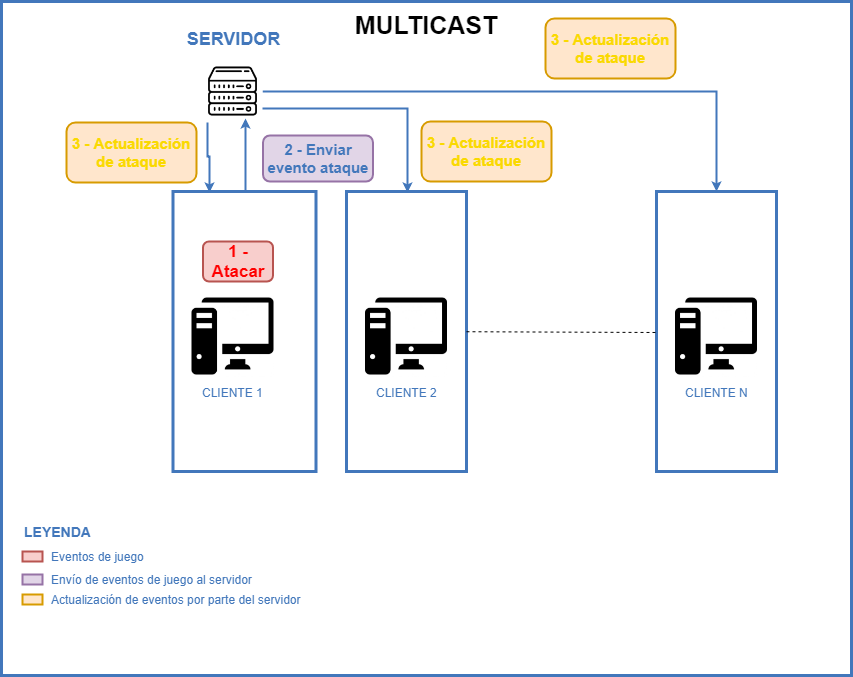
\includegraphics[width=13cm]{./images/Multicast.png}
  \caption{Esquema Multicast en \ac{UE4}}
  \label{Multicast}
\end{figure}
\end{itemize}

\subsubsection{\textit{Ownership}}

La posesión de un actor, es uno de los temas más importantes y que hay que tener más en cuenta a la hora de enfrentarse a un videojuego multijugador. Es importante ya que, como se ha comentado anteriormente, una llamada \ac{RPC} al servidor, se omitirá y no se ejecutará si se llama desde un cliente sobre un actor que no posee. 

Para resolver este problema, se ha seguido el esquema de la Figura \ref{Owning}, ya que la posesión de los actores recae en la instancia del jugador que reside en el servidor. Se comprueba si la llamada a \ac{RPC} del tipo NetMulticast se realiza desde una entidad autoritativa. En \ac{UE4} la autoridad la tiene quien \textit{spawnea} el actor. Si el actor es \textit{spawneado} desde un cliente, la autoridad la tendrá ese cliente. 

En el caso de \textit{Alliance}, los actores a replicar se \textit{spawnean} desde el servidor, y se replican a todos los clientes. Los actores que están colocados en el mundo desde el editor, se encuentran en la categoría <<\textit{placed in world}>>, distinta de la categoría <<\textit{spawned}>>, pero a efectos de replicación, estos actores se tratan como \textit{spawneados} en el servidor.

En el caso de que la llamada se haya realizado por una entidad autoritativa, se puede proceder a realizar la llamada a procedimiento remoto. Si no se ha realizado desde una entidad autoritativa, será necesario que se realice desde el \textit{owner} del actor, que como se ha dicho es la instancia del jugador en el servidor.

\begin{figure}[H]
  \centering
  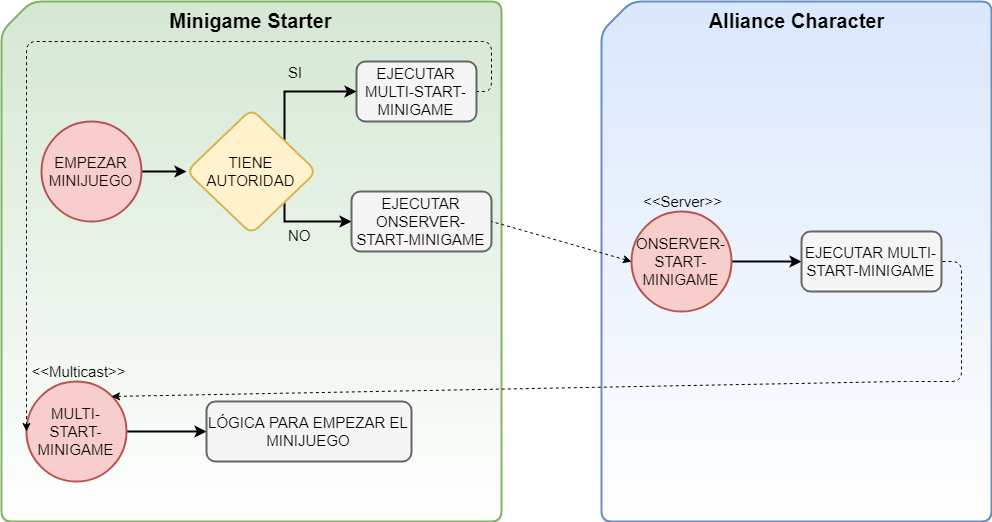
\includegraphics[width=13cm]{./images/Owning.png}
  \caption{\textit{Ownership} en \textit{Alliance}}
  \label{Owning}
\end{figure}
\end{itemize}

\subsubsection{El subsistema online en \ac{UE4}}

El subsistema online (\textit{Online Subsystem}) y sus interfaces, existen para proporcionar una abstracción clara de la funcionalidad online común en todo el conjunto de plataformas disponibles, como pueden ser Steam, Xbox Live, Facebook, etc. Se pretende conseguir principalmente la portabilidad.

Estas plataformas son necesarias, ya que proporcionan un servidor que se encarga de conectar los clientes con la lista de servidores o sesiones de juego disponibles. Además, permiten una visibilidad en internet, que un \textit{host} normalmente no tiene por sí mismo (por ejemplo, por falta de una dirección IP pública fija).

En \textit{Alliance} se ha hecho uso del subsistema online de Steam, por lo que para poder jugar será necesario tener Steam abierto. Al crear una nueva partida, el jugador que lo hace creará una sesión y será el \textit{host} de la partida. Una sesión es una instancia del juego, que se ejecuta en el servidor, con una serie de propiedades como pueden ser el número de jugadores que se aceptan en la partida, si los jugadores se pueden unir a la partida de forma pública o tienen que ser invitados para que puedan entrar, etc. 

Cuando un jugador se une a una partida, el subsistema online busca si existe alguna sesión creada que no se encuentre llena de jugadores. De ser así, pregunta al jugador si quiere unirse y en caso afirmativo, el jugador se une a la sesión que se ha encontrado (se puede ver el flujo de ejecución en el diagrama de la Figura \ref{seqOSS}). En este punto, la sesión estaría llena de jugadores (ya que en \textit{Alliance} se ha establecido un máximo de dos jugadores por sesión), el cliente que se ha unido pasaría a controlar al personaje no controlado por el \textit{host} de la partida, y ambos jugadores podrían comenzar a jugar juntos.

Para el cambio de niveles, se ha optado por destruir la sesión con el nivel actual y crear otra nueva a la que se unirán los dos jugadores. Se ha optado por este método ya que un servidor tiene la capacidad de alojar una sola sesión. Para permitir que se puedan unir varios jugadores a un mismo nivel, al abrir el nivel hay que indicar la opción <<\textit{listen}>>.

\begin{figure}[H]
  \centering
  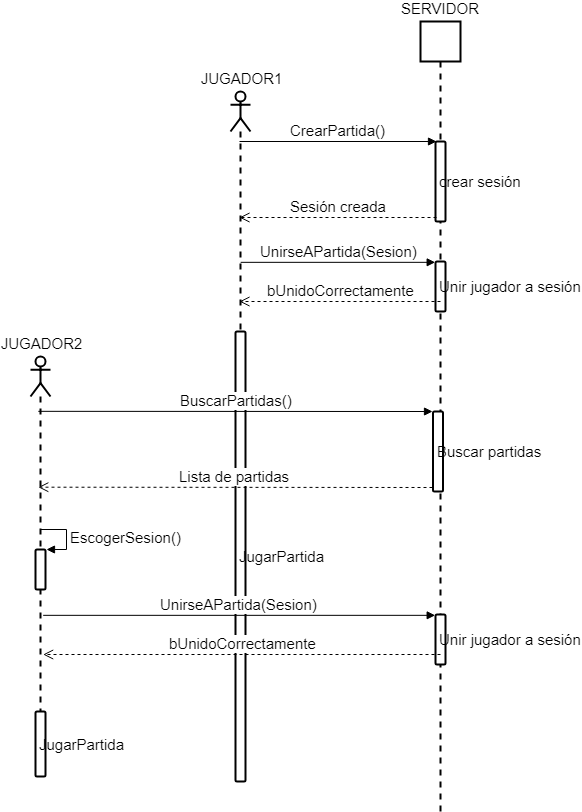
\includegraphics[width=10cm]{./images/Seq_OSS.png}
  \caption{Flujo de conexión de dos jugadores en una partida de \textit{Alliance}}
  \label{seqOSS}
\end{figure}
\end{itemize}

\subsubsection{Problemas que se han encontrado durante la replicación}

Durante el desarrollo de \textit{Alliance} ha habido algunos problemas relacionados con el multijugador y la replicación de los actores. Estos problemas han sido los más costosos de resolver, debido a la dificultad al depurar este tipo de problemas y la falta de información que se encontraba en foros de programación, como son StackOverflow\footnote{https://stackoverflow.com} y el foro de Unreal Engine\footnote{https://forums.unrealengine.com}. En muchos casos, era difícil seguir el flujo de ejecución del programa, por la naturaleza distribuida del videojuego. 

A continuación, se explican los problemas más notables y cómo se han afrontado en el proyecto:

\begin{itemize}
\item Como se ha visto anteriormente, para replicar un actor con apariencia de humano es necesario establecer las propiedades \texttt{bReplicates} y \texttt{bReplicateMovement}. Cuando se lanzaba el juego en multijugador, el jugador que actuaba como cliente (se llamará cliente al jugador que no actúa como \textit{host} y se llamará servidor al jugador que \textit{hostea} la partida) podía moverse pero cuando atacaba o esprintaba, el servidor no veía estos cambios. Para el servidor el jugador se seguía moviendo a velocidad normal y no veía que el cliente atacaba. 

Esto se producía debido a que las animaciones que se dan al esprintar o atacar no estaban siendo replicadas, ya que la llamada a un procedimiento \textit{multicast} desde un cliente, se ejecuta tan sólo localmente en dicho cliente y el comportamiento necesario es que se ejecute en el servidor, y se replique a cada uno de los clientes. Para resolverlo se tomó un enfoque basado en \ac{RPC}, de forma que cuando el cliente ataca, se notifica al servidor que se va a producir este ataque y el servidor se encarga de la replicación de la animación. Si es el servidor el que quiere atacar, se puede ejecutar de forma directa la llamada \ac{RPC} \textit{multicast}. Este enfoque, está basado en la Figura \ref{Owning}.

\item Problemas para lanzar el minijuego desde el cliente, debido a conflictos con el \textbf{ownership}. Cuando se intentaba lanzar el minijuego en el cliente, siguiendo un esquema como el de la Figura \ref{BadApproach}, nos encontrábamos con el problema de que el cliente no podía iniciar el minijuego. Esto es debido a que el enfoque que se siguió es erróneo. La función <<\textit{Server}>> nunca se ejecutaba, ya que era llamada desde un cliente que no es el \textit{owner} del actor, y como se ha explicado anteriormente, este tipo de llamadas se omiten y no se ejecutan.

Para resolverlo, se cambió el enfoque al de la Figura \ref{Owning}, de forma que ahora la función <<\textit{Server}>> sí es ejecutada, porque se llama en el \textit{owner} del actor, que como se ha dicho es la instancia del jugador en el servidor. Desde aquí se llama a la función <<\textit{Multicast}>>, replicando correctamente el funcionamiento.

\begin{figure}[H]
  \centering
  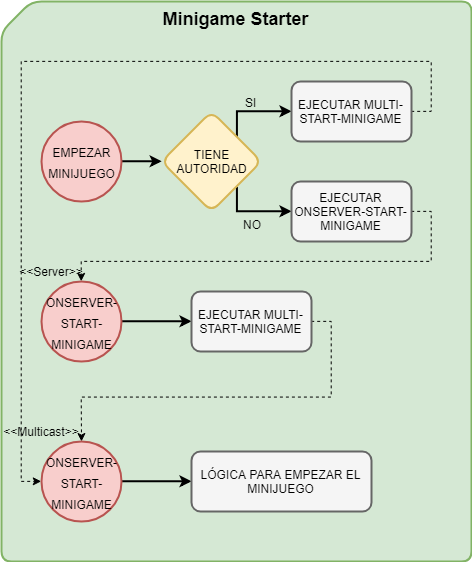
\includegraphics[width=7cm]{./images/BadApproach.png}
  \caption{Enfoque incorrecto al lanzar el minijuego desde el cliente}
  \label{BadApproach}
\end{figure}

\item \textit{Crasheo} del videojuego por un error de violación de segmentos en tiempo de ejecución. Este \textit{crasheo} ocurría al jugar el minijuego cuando un jugador lo había jugado anteriormente.

El error venía causado porque se accedía a una referencia local desde una máquina remota (no tiene sentido compartir una referencia a memoria a un jugador remoto, ya que la memoria de ambos es completamente distinta). Este problema era causado en el evento \texttt{BeginOverlap}. En este evento se toma una referencia al jugador que está haciendo \textit{overlap} (que será quien juega el minijuego), y este evento parecía ejecutarse varias veces, con un comportamiento parecido al de un evento <<\textit{Multicast}>>.

Tras emplear mucho tiempo intentando buscar la solución al problema (para conseguir el comportamiento que se observa en la Tabla \ref{Behaviour}) y no conseguir arreglarlo, se optó por deshabilitar de forma temporal la posibilidad de que el cliente jugase el minijuego, limitando la jugabilidad del mismo al servidor (véase la Figura \ref{Limitation}). Esta no es una opción definitiva (que el cliente pueda jugar el minijuego es una característica muy deseable), por lo que este error se solucionará en actualizaciones futuras. Sin embargo, por el momento no supone un gran problema, ya que aunque el cliente no pueda jugar el minijuego, si que puede observar cómo el servidor lo juega.

\begin{table}[H]
\centering
\begin{tabular}{|c|c|}
\hline
\textbf{Quién juega el minijuego} & \textbf{Comportamiento Deseado}        \\ \hline
Servidor                          & El cliente no puede jugarlo a la vez   \\ \hline
Cliente                           & El servidor no puede jugarlo a la vez  \\ \hline
Cualquiera lo ha jugado           & El minijuego no puede volver a jugarse \\ \hline
\end{tabular}
\caption{Comportamiento deseado del minijuego}
\label{Behaviour}
\end{table}

\begin{figure}[H]
  \centering
  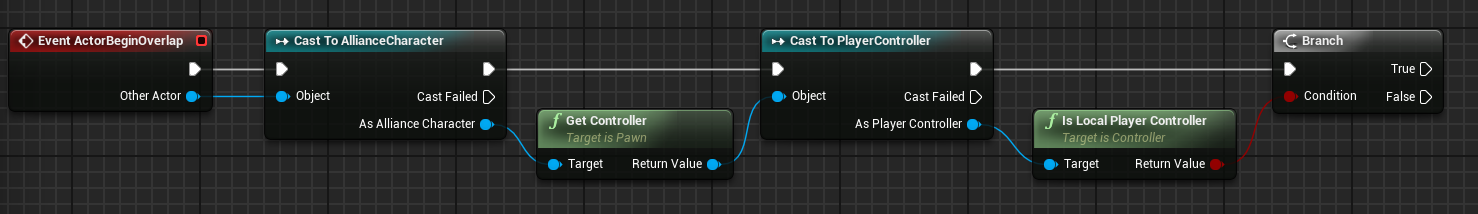
\includegraphics[width=13cm]{./images/LimitacionMinijuego.png}
  \caption{Limitación en la ejecución del minijuego a solo el servidor}
  \label{Limitation}
\end{figure}
\end{itemize}

\subsection{Patrón Observador y Patrón Factoría en la creación de enemigos}

Para \textit{spawnear} los enemigos en el juego, se ha usado un actor a modo de \textit{spawner}, que se encargará de crear los enemigos de cada tipo que se indican por medio de propiedades en el editor. Recibe también como parámetro el número de oleadas de enemigos que aparecerán. Se ha diseñado un esquema basado en el patrón factoría para el \textit{spawn} de los enemigos y basado en el patrón observador para detectar cuando los enemigos de un cierto \textit{spawner} han muerto.

Para crear los enemigos, se usa un \textit{spawner} que comenzará la creación cuando el jugador alcanza una cierta zona del mapa (mediante \textit{overlap} con alguna caja de colisiones invisible). El \textit{spawner} sabe cuántos enemigos de cada tipo tiene que \textit{spawnear} y cuantas oleadas lanzará, pero la creación de los enemigos recae sobre una factoría de enemigos (véase la Figura \ref{Factory}). Esta factoría es la encargada de colocar sobre una determinada posición del mundo a un enemigo de un tipo indicado por el \textit{spawner} y devolverle al mismo el enemigo creado.

 
\begin{figure}[H]
  \centering
  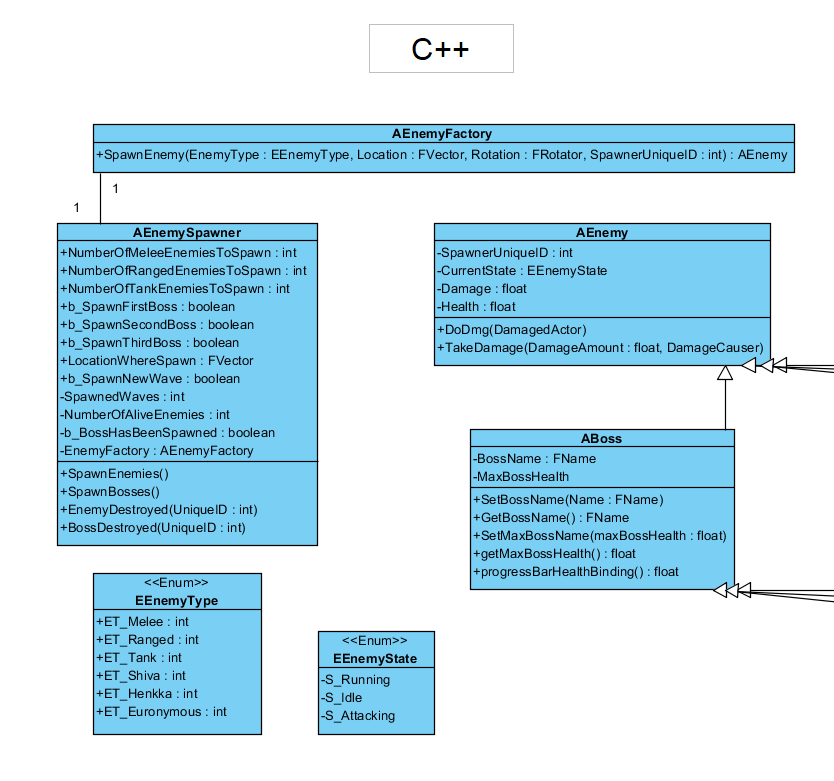
\includegraphics[width=11cm]{./images/FactoryPattern.png}
  \caption{Patrón factoría para la creación de enemigos}
  \label{Factory}
\end{figure}

Para que el \textit{spawner} sepa cuándo un enemigo que ha creado él ha sido eliminado, se usa el patrón observador con delegados (ver Figura \ref{Observer}). En la creación de enemigos, cuando la factoría crea un enemigo, le indica un identificador único que se corresponde con el identificador del \textit{spawner} que lo ha creado. De esta forma, cuando un enemigo muere, notifica mediante el delegado a todos los observadores que ha muerto, usando el identificador que se le ha otorgado. Los \textit{spawner} comprueban si el enemigo que ha muerto ha sido creado por ellos, por medio de este identificador, y de ser así, decrementan su contador de enemigos vivos.

Si este contador llega a cero, significará que todos los enemigos que han creado han sido eliminados. Si quedan mas rondas de enemigos por \textit{spawnear}, procederán a lanzar una nueva ronda de enemigos. Si por el contrario, las rondas de enemigos que el \textit{spawner} tiene que lanzar han sido lanzadas, el \textit{spawner} se destruirá, ya que su labor no es necesaria.

Para acceder a ciertas zonas del mapa que están bloqueadas, es necesario que se hayan eliminado los enemigos de las zonas anteriores. Para llevar a cabo esta comprobación, se mira que los \textit{spawners} de las zonas anteriores hayan sido destruidos. Como se ha dicho, los \textit{spawners} se destruyen una vez que éstos no tienen más enemigos que crear y los que han creado han muerto. Si la comprobación de que los \textit{spawners} de las zonas anteriores están destruidos es cierta, significará que todos los enemigos hasta el momento han muerto.

\begin{figure}[H]
  \centering
  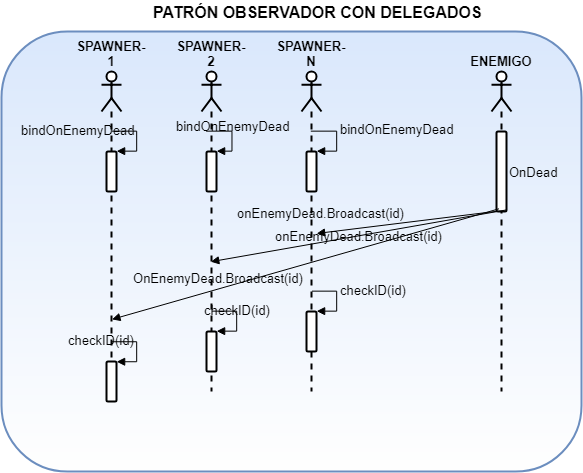
\includegraphics[width=10cm]{./images/Observer.png}
  \caption{Patrón observador en la destrucción de enemigos}
  \label{Observer}
\end{figure}

\subsection{Diálogos en \textit{Alliance}}

Para implementar los diálogos en \textit{Alliance} se ha optado por usar un \textit{plugin}, debido a que el proyecto quedaría mucho más limpio de esta forma y además se ha conseguido un ahorro de tiempo considerable en el desarrollo del proyecto, junto con la facilidad al maquetar los diálogos. El \textit{plugin} se llama \textit{NotYetDialogueSystem} y se puede encontrar de forma gratuita en el \textit{marketplace} de \ac{UE4}\footnote{https://www.unrealengine.com/marketplace/not-yet-dialogue-system}. Se trata de un \textit{plugin} para realizar los diálogos muy potente, basado en una estructura en forma de árbol y orientado a participantes. Esta estructura en forma de árbol se ejecutará de acuerdo a condiciones, que se establecen en los nodos del árbol. Existen varios tipos de nodos, pero los que se han usado para los diálogos de \textit{Alliance} son los nodos de <<discurso>> (o \textit{speech}). A este tipo de nodos se le indica qué texto se mostrará en el diálogo. Entre otras opciones interesantes, cabe destacar el posible uso de archivos de audio en el diálogo, que se reproducirán durante el mismo.

Para establecer los diálogos, es necesario implementar la interfaz que se puede observar en la Figura \ref{Dialog} en la clase del actor participante en el diálogo. Todos los actores que participen en un diálogo deben tener implementada esta interfaz. Una vez que se ha realizado dicha implementación, se pueden usar Blueprints para maquetar estos diálogos, con una estructura en forma de árbol. Aunque se puede hacer el árbol todo lo complejo que se quiera, introduciendo nodos de condición, en \textit{Alliance} se ha optado por seguir una ejecución secuencial, debido a que no era necesario realizar diálogos tan complejos.

Para lanzar los diálogos durante la ejecución del juego, se han usado dos enfoques:

\begin{itemize}
\item Mostrar los diálogos cuando se produce un determinado evento, como puede ser que se haya completado el minijuego correctamente, que se haya eliminado a un jefe final, etc.
\item Mostrar los diálogos cuando se llega a una parte específica del mapa, al hacer \textit{overlap} con alguna caja de colisiones invisible. 
\end{itemize}

\begin{figure}[H]
  \centering
  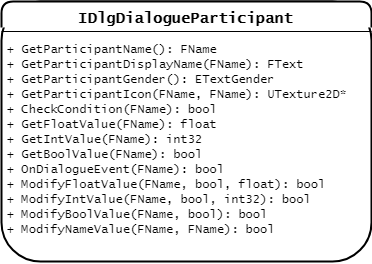
\includegraphics[width=7cm]{./images/IDlgParticipant.png}
  \caption{Interfaz que tienen que implementar los participantes en un diálogo}
  \label{Dialog}
\end{figure}

\subsection{\textit{Breakables} y \textit{Pickups}}

Con el objetivo de incrementar la jugabilidad y teniendo en cuenta que el combate es muy importante en el juego, se ha querido introducir en \textit{Alliance} un mecanismo para conseguir aumentar la vida y la estamina del jugador, mediante la destrucción de ciertos objetos decorativos que se encuentran en el mapa, como son cajas, barriles, carros, etc. 

Estos objetos se han implementado completamente en C++ y otorgan la posibilidad de \textit{spawnear} \textit{pickups} de vida, de estamina o simplemente no \textit{spawnear} nada cuando se rompen. Los objetos decorativos se rompen cuando \textit{Alyssa} ataca con su maza, colisionando con estos objetos o cuando \textit{Morten} dispara sobre los mismos, usando sus armas. Sin embargo, estos objetos no se rompen con los ataques especiales de los personajes, la bola de fuego en el caso de \textit{Alyssa} y la granada en el caso de \textit{Morten}. 

Cabe destacar que ambos actores están completamente replicados, por lo que si el cliente rompe un objeto, el servidor no podrá volver a romperlo ya que observará que ya se encuentra roto (y viceversa). Para conseguir esto, se ha hecho uso de \ac{RPC}, que se ha comentado anteriormente.

La probabilidad de que cuando se rompe un \textit{breakable} se \textit{spawnee} algún objeto de vida o de estamina, se puede poner desde el editor. Se ha hecho así ya que puede ser útil que en un \textit{breakable} concreto se \textit{spawnee} un tipo fijo de \textit{pickup}, por ejemplo el \textit{spawn} de vida en un objeto que se encuentra en un área de combate con jefes enemigos, o el \textit{spawn} de estamina en objetos que se encuentran en los caminos de transición entre distintas arenas. 

Cuando se rompe un \textit{breakable}, al igual que cuando se coge un \textit{pickup} se reproduce un sonido. A estos sonidos, al igual que a los sonidos de los enemigos y personajes, se les ha añadido una atenuación con la distancia, de forma que cuanto más se aleje el personaje de la fuente del sonido, más suaves oirá estos sonidos. Si el personaje está suficientemente lejos, dejará de oír los sonidos gracias a la atenuación. 